\documentclass[11pt,a4paper]{article}
\usepackage[left=2cm,text={17cm,25cm},top=2.5cm]{geometry}
\usepackage[T1]{fontenc}
\usepackage[czech]{babel}
\usepackage[utf8]{inputenc}
\usepackage{url}
\usepackage{graphicx}
\usepackage{pdfpages}
\usepackage[colorinlistoftodos,prependcaption,textsize=tiny]{todonotes}

\graphicspath{ {figs/} }

\begin{document}

\begin{center}
	\LARGE{SIN -- Inteligentní systémy}\\
	\Large{Implementace meteostanice s autonomním řízením}
	\vspace{0.5cm}

    \begin{centering}
        \small{Bc. Petr Stehlík <xstehl14@stud.fit.vutbr.cz>}
    \end{centering}

    \begin{centering}
        \small{Bc. Matej Vido <xvidom00@stud.fit.vutbr.cz>}
    \end{centering}

	\vspace{0.2cm}

\end{center}

\section{Úvod}
Cílem projektu je navrhnout a implementovat meteostanici využívající MQTT protokol pro zasílání naměřených hodnot serveru. Server implementuje databázi a webové grafické uživatelské rozhraní (GUI), analyzuje historické hodnoty a na jejich základě řídí akce aktuátorů.

Meteostanice měří teplotu, vlhkost a tlak vzduchu; vlhkost v květináči a světelnou intenzitu. Navržené aktuátory jsou ovládání žaluzií, klimatizace, topení a zavlažování rostlin. Vše je autonomně ovládáno na základě předem stanovených pravidel.

GUI zobrazuje aktuální a historické naměřené hodnoty jednotlivých senzorů, trendy a naposledy vykonané akce aktuátorů společně s krátkodobou předpovědí počasí získanou z volně dostupných zdrojů.

\section{Nástroje pro monitoring a řízení}
Na trhu je velké množství dostupných nástrojů pro monitoring a řízení a to i na poli chytrých domácností. Je zde mnoho komerčních a uzavřených systémů pro automatizaci domácnosti. V současnosti nejznámější a pravděpodobně i nejrozšířenější je Apple Home\footnote{\url{https://www.apple.com/lae/ios/home/}}, který využívá protokolu Homekit také od společnosti Apple. Na trhu existuje pro Apple Home velké množství produktů a neustále se jejich počet zvyšuje. Existuje ale i mnoho open-source nástrojů pro řízení domácnosti. Jejich nejrozšířenější zastupitele jsou zde v krátkosti popsány.

\subsection{Grafana}
Grafana\footnote{\url{https://grafana.com/}} je vizualizační a analytický nástroj pro data zachycená v čase. Grafana samotná není primárně určena pro monitoring a řízení chytrých domácností, ale je natolik upravitelná, že existují konfigurace, které toto užití zpřístupňují. Je dostupná s mnoha rozšířeními a zdroji dat. Uživatel si vytvoří dashboard, který si následně nakonfiguruje a seskládá z dostupných modulů. Tyto moduly mimo dalších funkcionalit umožňují zobrazit čárový graf, jednotlivé hodnoty, trendy hodnot a s pomocí modulů i různé přepínače.

\subsection{Domoticz}
Domoticz\footnote{\url{https://domoticz.com/}} je kompletním open-source systémem pro domácí automatizaci. Tento nástroj dovoluje monitorovat, řídit a konfigurovat mnoho různých zařízení od různých výrobců. Disponuje i automatickým učením senzorů a aktuátorů. Rozhraní pro uživatele je vytvořeno jako webová stránka dostupná na stroji s lokální instalací Domoticz.

\subsection{OpenHAB}
OpenHAB\footnote{\url{https://www.openhab.org/}} je dalším velmi známým zástupcem open-source nástrojem pro domácí automatizaci. Podporuje velké množství platforem, výrobců a zařízení. Dokáže integrovat mnoho systémů do jednoho centrálního řešení, které lze ovládat mobilní aplikací, webových rozhraním nebo nativní desktopovou aplikací. Pro automatizaci disponuje rozsáhlým systémem pro tvorbu komplexních pravidel.

\subsection{Home Assistant}
Home Assistant\footnote{\url{https://home-assistant.io/}} je primárně navrhován pro užívání na Raspberry Pi. Jako předchozí nástroje také podporuje široké množství výrobců a zařízení. Také disponuje konfigurovatelným webových rozhraním s přehledy zařízení a kontrolou aktuátorů.

\subsection{BeeeOn}
BeeeOn\footnote{\url{https://beeeon.org/wiki/Main\_Page}} je systém pro domácí automatizaci vyvíjený na FIT VUT v Brně. Tento systém je primárně vyvíjen jako bezpečná domácí brána pro různé IoT zařízení. Oproti předchozím systémům je nutno pro plnou funkcionalitu systému vlastnit domácí bránu, kterou lze propojit s několika výrobci a jejich zařízeními. BeeeOn disponuje Android mobilní aplikací pro ovládání domácnosti a prototypem webového rozhraní.

\subsection{Vlastní řešení}
%TODO do cestiny
Okrem uvedených kompletných riešení pre monitoring a analýzu riadiachich systémov je možné poskladať vlastné riešenie
z dostupných open-source knižníc, frameworkov a nástrojov.

Rozšíreným frameworkom pre tvorbu klientskej časti webových aplikácií je Angular\footnote{\url{https://angular.io/}}.
Angular napísaný v jazyku TypeScript umožňuje jednoduchú integráciu rôznych knižníc pre zobrazovanie grafov a tvorbu dashboardov.

K implementácii serverovej časti webovej aplikácie je možné použiť framework Flask\footnote{\url{http://flask.pocoo.org/}} v jazyku Python.
Flask umožňuje rýchlu a jednoduchú tvorbu REST API na prepojenie serverovej a klientskej časti webovej aplikácie.
Výhodou použitia jazyku Python pre tvorbu serverovej časti aplikácie je, že obsahuje moduly pre obsluhu databázového systému
a zabezpečenie sieťovej komunikácie s ďalšími prvkami celého riadiaceho systému.

Mosquitto\footnote{\url{https://mosquitto.org/}} je voľne dostupný broker pre MQTT protokol používaný v prostredí systémov IoT podporujúci rôzne platformy.

\section{Architektura a implementace}
%TODO do cestiny
V tejto sekcii je popísaná architektúra a implementácia vytvorenej meteostanice s autonómnym riadením.
Meteostanica obsahuje reálne senzory, z ktorých sú dáta prenášané na server.
Server dáta ukladá do databázy, riadi činnosť aktuátorov podľa pravidiel, ktoré sú taktiež uložené v databáze,
a obsluhuje webovú aplikáciu, ktorá poskytuje grafické užívateľské rozhranie k celému systému.
Činnosť aktuátorov je simulovaná.
Pre účely testovania bol taktiež zostrojený modul pre simulovanie činnosti senzorov.
V časti~\ref{subsec:hw} je popísaný hardware a spôsob jeho zapojenia.
V nasledujúcej časti~\ref{subsec:sw} je popísaná implementácia softwareových modulov systému.

\subsection{Hardware}\label{subsec:hw}
Základem pro hardware byly zvoleny Raspberry Pi 2 jako server a Raspberry Pi Zero W jako samotná meteostanice. Server realizován jako Raspberry Pi 2 zpřístupňuje uživateli minimalistické webové rozhraní a slouží jako MQTT broker pro meteostanici. Také jsou zde ukládány všechny naměřené hodnoty do SQLite3 databáze.
Na obrázku~\ref{fig:hw-scheme} je znázornená schéma zapojenia senzorov a Raspberry Pi.

K Raspberry Pi Zero W jsou připojeny následující senzory:

\begin{itemize}
    \item DHT11 - digitální senzor pro měření teploty a vlhkosti vzduchu
    \item BMP180 - digitální senzor pro měření barometrického tlaku, teploty a nadmořské výšky
    \item TEMT6000 - analogový senzor pro měření intenzity okolního světla
    \item YL-69 společně s YL-38 - analogový senzor pro měření vlhkosti půdy
\end{itemize}

Pro konverzi analogových senzorů je použit AD převodník MCP3008.

\begin{figure}[htb]
    \centering
    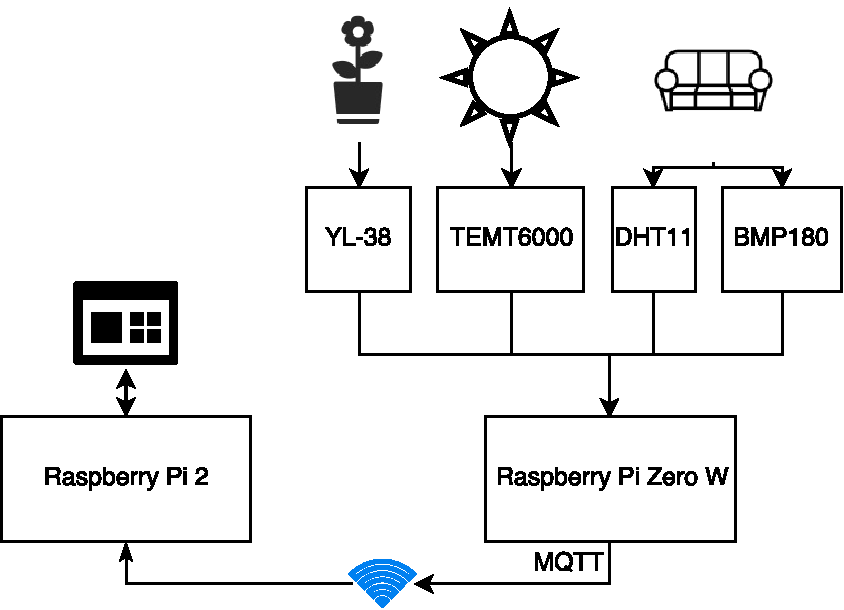
\includegraphics[width=0.5\linewidth]{weather-station-scheme}
    \caption{Schéma zapojenia hardware.}
\end{figure}

\subsection{Software}\label{subsec:sw}

V tejto časti sú popísané naimplementované časti software a nástroje použité
k činnosti meteostanice s autonómnym riadením.
Na obrázku~\ref{fig:sw-scheme} je znázornené prepojenie jednotlivých modulov
a spôsob ich komunikácie.

\begin{figure}[htb]
    \label{fig:sw-scheme}
    \centering
    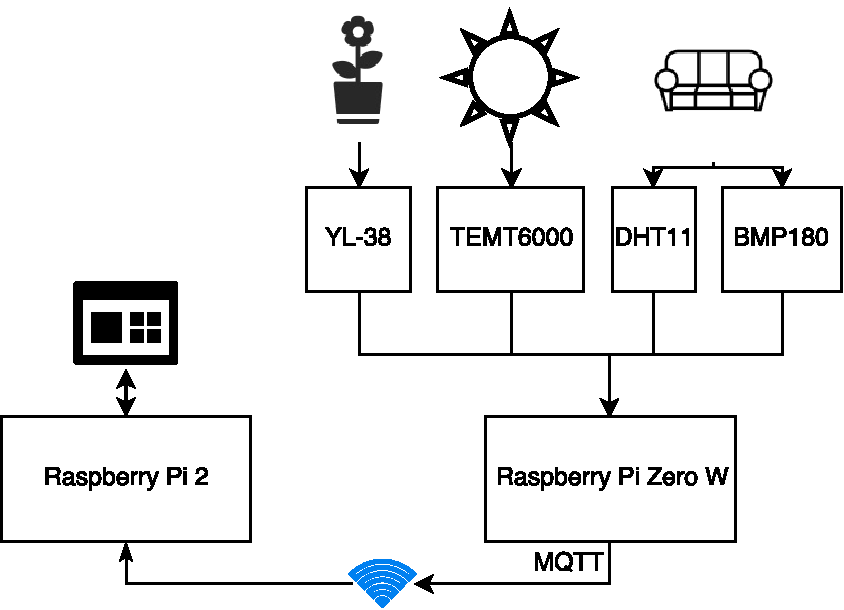
\includegraphics[width=0.5\linewidth]{weather-station-scheme}
    \caption{Schéma prepojenia softwareových modulov.}
\end{figure}

Interakciu s užívateľom sprostredkúva webová aplikácia, ktorá sa skladá z grafického
užívateľského rozhrania (GUI) zobrazovaného vo webovom prehliadači a serverovej časti.

Webové grafické užívateľské rozhranie je naimplementované vo frameworku Angular verzie 4.
\todo[inline]{krátky popis angularu, kniznic pouzitych na zobrazenie grafov}
GUI zobrazuje dáta prenášané zo serveru prostredníctvom REST API.

Serverová časť webovej aplikácie (backend) prijíma dáta zo senzorov a ukladá ich do databázy.
Na základe dát zo senzorov a nastavených pravidiel určuje činnosť aktuátorov, a komunikuje s aktuátormi.
Backend je naimplementovaný v jazyku Python.
K implementácii REST API je použitý framework Flask.
\todo[inline]{kratky popis flasku}
REST API umožňuje:
\begin{itemize}
    \item získať poslednú vzorku dát zo senzorov vrátane časovej známky spolu s trendom vypočítaným
        pre každú meranú veličinu
    \item získať informácie o aktuálnom stave aktuátorov a pravidlách, ktorými sú riadené
\end{itemize}

Výpočet trendov prebieha na základe lineárnej aproximácie z určitého počtu posledných vzoriek danej veličiny.
Pre každú veličinu je tak určená funkcia v tvare:
\[
    y = a x + b
\]
Koeficient $a$ udáva ako prudko funkcia klesá alebo stúpa.
Koeficient $b$ udáva posunutie funkcie po osi $x$.
Toto posunutie nemá na zmenu veličiny vplyv a preto môže byť z ďalších výpočtov vypustené.
Do vzťahu:
\[
    y = a x
\]
je potom za $x$ dosadený počet vzoriek, z ktorých sa počíta trend.
Hodnota $y$ udáva o koľko sa daná veličina za posledných $x$ vzoriek zmenila.
Pre každú veličinu boli empiricky určené hodnoty prahov.
Ak je absolútna hodnota zmeny veličiny väčšia ako prah,
podľa znamienka zmeny veličiny je určený stúpajúci alebo klesajúci trend,
inak je určený trend rovnomerného priebehu.

Pre ukladanie dát je použitý databázový systém SQLite3, ktorého výhodou je jeho jednoduchosť
a štandardná podpora v jazyku Python.
Dátabázové dáta sú uložené v jedinom súbore.
V databáze sa nachádzajú 3 tabuľky:
\begin{itemize}
    \item \texttt{weather\_data} - obsahuje históriu dát zo senzorov
    \item \texttt{actuators} - obsahuje informácie o stave aktuátorov
    \item \texttt{thresholds} - obsahuje informácie o pravidlách riadiacich činnosť aktuátorov
\end{itemize}

Dáta zo senzorov získava, agreguje a následne odosiela backendu modul \texttt{sensors}.
Pre testovacie účely bol pripravený aj modul \texttt{fake-sensors}, ktorý simuluje
činnosť modulu \texttt{sensors} a odosiela umelé dáta v rovnakom formáte.

Modul \texttt{fake-actuators} simuluje činnosť aktuátorov.
Z backendu prijíma príkazy na zmenu stavu aktuátorov, ktoré simuluje.
Po prevedení činnosti aktuátoru je odoslaná informácia o stave, v ktorom
sa aktuátor nachádza backendu.
Nasleduje zoznam simulovaných aktuátorov:
\begin{itemize}
    \item klimatizácia - riadená na základe údajov o teplote
    \item kúrenie - riadené na základe údajov o teplote
    \item žalúzie - riadené na základe údajov o intenzite svetla
    \item zavlažovanie rastlín - riadené na základe údajov o vlhkosti pôdy
\end{itemize}

Komunikácia medzi backendom, senzormi a aktuátormi prebieha cez protokol MQTT.
\todo[inline]{kratky popis MQTT}
Ako broker je použité Mosquitto.

\section{Výsledky}\label{sec:res}

\section{Závěr}\label{sec:sum}

\end{document}
